% First comes an example EPS file -- just ignore it and
% proceed on the \documentclass line
% your LaTeX will extract the file if required
%\begin{filecontents*}{example.eps}
%!PS-Adobe-3.0 EPSF-3.0
%%BoundingBox: 19 19 221 221
%%CreationDate: Mon Sep 29 1997
%%Creator: programmed by hand (JK)
%%EndComments
%gsave
%newpath
%  20 20 moveto
%  20 220 lineto
%  220 220 lineto
%  220 20 lineto
%closepath
%2 setlinewidth
%gsave
%  .4 setgray fill
%grestore
%stroke
%grestore
%\end{filecontents*}



\RequirePackage{fix-cm}

%\documentclass[smallextended]{./springer/svjour3}       % onecolumn (second format)
%% \smartqed  % flush right qed marks, e.g. at end of proof

\usepackage{amsmath}
\usepackage{amsfonts}

% Russian-specific packages
%--------------------------------------
\usepackage[T2A]{fontenc}
\usepackage[utf8]{inputenc}
\usepackage[russian]{babel}
%--------------------------------------

% Asymptote for pictures
%--------------------------------------
\usepackage{asymptote} %% comes with options inline and attach
%--------------------------------------

% graphicx for graphs
%--------------------------------------
\usepackage{graphicx}

%--------------------------------------
% Specially for PMM: make all imported EPS grayscale:
%--------------------------------------
\usepackage[gray]{epspdfconversion}
%--------------------------------------

% \usepackage{subfig} % incompatible with subcaption package
% \graphicspath{ % not used here
    % {./pic/,./asy/}
% }
%--------------------------------------

% subcaption for many figures under one big caption
% each having its own small caption
%--------------------------------------
\usepackage{caption}
\usepackage{subcaption}
%--------------------------------------

% so that refs were [1-10], not [1,2,3,4,5,...]
%--------------------------------------
\usepackage{cite}
%--------------------------------------

% \ddfrac command to show big fractions, not cramped up
% https://tex.stackexchange.com/questions/173899/
%--------------------------------------
\newcommand\ddfrac[2]{\displaystyle\frac{\displaystyle #1}{\displaystyle #2}}
%--------------------------------------

% \vsp command to make a spacey newline
% useful for equations arrays
%--------------------------------------
\newcommand\vsp[1][10]{\\[#1pt]}
%--------------------------------------

% partial derivatives (can \usepackage{physics}, but only one command so far, so no)
%--------------------------------------
\newcommand\pd[2]{\frac{\partial #1}{\partial #2}}
\newcommand\ddpd[2]{\ddfrac{\partial #1}{\partial #2}}
\newcommand\ddt[1]{\frac{d #1}{dt}}
\newcommand\ddddt[1]{\ddfrac{d #1}{dt}}
%--------------------------------------

% unbreakable space parenthesized reference
%--------------------------------------
\newcommand\upr[1]{~(\ref{#1})}
%--------------------------------------

% Nice letters
%--------------------------------------
\newcommand\M[0]{\mathcal{M}} % Matrix of intertia
\newcommand\AntiU[0]{\mathcal{U}} % Helper antisymmetric matrix for eqs' RHS
\newcommand\Rhs[0]{\mathcal{R}} % RHS
\newcommand\Prhs[0]{\mathcal{P}} % The family of matrices for RHS
\newcommand\prhs[0]{\mathbf{p}} % Poisson brackets
%--------------------------------------

\renewcommand{\vec}[1]{\boldsymbol{\mathbf{#1}}}

\newtheorem{stmt}{Утверждение}
\newtheorem{prblm}{Затруднение}

% --------------------------------------------------------------
% ТИТУЛЬНЫЙ ЛИСТ И АННОТАЦИЯ
% --------------------------------------------------------------

%\begin{document}

%\title{Движение симметричного экипажа на омни-колесах\\с массивными роликами}

%\author{Герасимов К.В. \and
%        Зобова А.А
%}

%\institute{Кафедра теоретической механики и мехатроники\\
%Механико-математический факультет\\
%МГУ им. М.В. Ломоносова \at
%              Москва\\
%              Тел.: (495) 939-36-81\\
%              \email{kiriger@gmail.com, azobova@gmail.com}
%}

%\maketitle

%\begin{abstract}
%Рассматривается динамика симметричного экипажа с роликонесущими колесами, движущегося по  неподвижной горизонтальной абсолютно шероховатой плоскости в следующих предположениях: масса каждого ролика ненулевая, контакт между роликами и плоскостью точечный, проскальзывания нет. Уравнения движения составлены с помощью системы символьных вычислений Maxima. В уравнениях движения выявлены дополнительные члены, пропорциональные собственному моменту инерции ролика. Эти слагаемые явно зависят от углов поворота колес. Вследствие этого, для замыкания системы уравнений необходимо добавить уравнения связей. Предложена модель перехода колеса с одного ролика на другой, при этом разрывы в правых частях уравнений движения устранены путем введения дополнительных предположений о характере движения роликов. Показано, что ряд движений, существующих в безынерционной модели (т.е. не учитывающей массу роликов), пропадает, так же как и линейный первый интеграл. Проведено сравнение основных типов движения симметричного трехколесного экипажа, полученных численным интегрированием уравнений движения с безынерционной моделью. 

%Ключевые слова: омни-колеса, роликонесущие колеса, лаконичная форма уравнений движения Я.В. Татаринова

%\end{abstract}

%\newpage



\documentclass[12pt]{extarticle}
% \smartqed  % flush right qed marks, e.g. at end of proof

\usepackage{amsmath}
\usepackage{amsfonts}

% Russian-specific packages
%--------------------------------------
\usepackage[T2A]{fontenc}
\usepackage[utf8]{inputenc}
\usepackage[russian]{babel}
%--------------------------------------

% Asymptote for pictures
%--------------------------------------
\usepackage{asymptote} %% comes with options inline and attach
%--------------------------------------

% graphicx for graphs
%--------------------------------------
\usepackage{graphicx}

%--------------------------------------
% Specially for PMM: make all imported EPS grayscale:
%--------------------------------------
\usepackage[gray]{epspdfconversion}
%--------------------------------------

% \usepackage{subfig} % incompatible with subcaption package
% \graphicspath{ % not used here
    % {./pic/,./asy/}
% }
%--------------------------------------

% subcaption for many figures under one big caption
% each having its own small caption
%--------------------------------------
\usepackage{caption}
\usepackage{subcaption}
%--------------------------------------

% so that refs were [1-10], not [1,2,3,4,5,...]
%--------------------------------------
\usepackage{cite}
%--------------------------------------

% \ddfrac command to show big fractions, not cramped up
% https://tex.stackexchange.com/questions/173899/
%--------------------------------------
\newcommand\ddfrac[2]{\displaystyle\frac{\displaystyle #1}{\displaystyle #2}}
%--------------------------------------

% \vsp command to make a spacey newline
% useful for equations arrays
%--------------------------------------
\newcommand\vsp[1][10]{\\[#1pt]}
%--------------------------------------

% partial derivatives (can \usepackage{physics}, but only one command so far, so no)
%--------------------------------------
\newcommand\pd[2]{\frac{\partial #1}{\partial #2}}
\newcommand\ddpd[2]{\ddfrac{\partial #1}{\partial #2}}
\newcommand\ddt[1]{\frac{d #1}{dt}}
\newcommand\ddddt[1]{\ddfrac{d #1}{dt}}
%--------------------------------------

% unbreakable space parenthesized reference
%--------------------------------------
\newcommand\upr[1]{~(\ref{#1})}
%--------------------------------------

% Nice letters
%--------------------------------------
\newcommand\M[0]{\mathcal{M}} % Matrix of intertia
\newcommand\AntiU[0]{\mathcal{U}} % Helper antisymmetric matrix for eqs' RHS
\newcommand\Rhs[0]{\mathcal{R}} % RHS
\newcommand\Prhs[0]{\mathcal{P}} % The family of matrices for RHS
\newcommand\prhs[0]{\mathbf{p}} % Poisson brackets
%--------------------------------------

\renewcommand{\vec}[1]{\boldsymbol{\mathbf{#1}}}

\newtheorem{stmt}{Утверждение}
\newtheorem{prblm}{Затруднение}

\voffset=-15mm \textwidth=17cm \textheight=24cm
\oddsidemargin=0cm \topmargin=+0cm \headsep=10pt \evensidemargin=0mm
\renewcommand{\baselinestretch}{2}

\makeatletter \@addtoreset{equation}{section} \makeatother
\makeatletter
\renewcommand{\@biblabel}[1]{#1. \hfill}
\makeatother


\renewcommand{\thesection}{\arabic{section}}
\renewcommand{\theequation}{\arabic{section}.\arabic{equation}}
\renewcommand{\refname}{}

\begin{document}

\begin{flushleft}
УДК 531.01
\end{flushleft}

\begin{center}
\Large К.В. Герасимов, А.А. Зобова

Движение симметричного экипажа на омни-колесах с массивными роликами


\vspace{1cm}
\parbox{14cm}{
    \normalsize
    \hspace{1cm} Рассматривается динамика симметричного экипажа с роликонесущими колесами, движущегося по  неподвижной горизонтальной абсолютно шероховатой плоскости в следующих предположениях: масса каждого ролика ненулевая, контакт между роликами и плоскостью точечный, проскальзывания нет. Уравнения движения составлены с помощью системы символьных вычислений Maxima. В уравнениях движения получены дополнительные члены, пропорциональные осевому моменту инерции ролика и зависящие от углов поворота колес. Массивность роликов учитывается в тех фазах движения, когда не происходит смены роликов в контакте. При переходе колес с одного ролика на другой масса роликов считается пренебрежимо малой. Показано, что ряд движений, существующих в безынерционной модели (т.е. не учитывающей массу роликов), пропадает, так же как и линейный первый интеграл. Проведено сравнение основных типов движения симметричного трехколесного экипажа, полученных численным интегрированием уравнений движения с результатами, полученными на основании безынерционной модели.
}
\vspace{1.5cm}
\end{center}


% --------------------------------------------------------------
% ОСНОВНОЙ МАТЕРИАЛ
% --------------------------------------------------------------

\chapter{Динамика экипажа на омни-колесах с трением}

В предыдущих главах рассмотрена динамика омни-колесного экипажа на абсолютно шероховатой плоскости. Однако, как было показано ранее, в этом случае на интервалах движения без смены ролика в контакте полная механическая энергия сохраняется, что никогда не происходит в реальных системах. Отдельного рассмотрения заслуживает вопрос о том, прекращается ли в реальных системах скольжение вновь вошедшего в контакт ролика. Таким образом, 
интерес представляет изучение динамики экипажа по плоскости с трением.

В данной главе вместо идеальных неголомных связей отсутствия проскальзывания используются голономные неидеальные неудерживающие связи. Для касательных составляющих реакций опорной плоскости используются две модели: сухое трение Амонтона -- Кулона, регуляризованного в окрестности нуля по скорости проскальзывания линейной функцией с насыщением; вязкое трением.

Построение модели выполнено таким образом, что изменение в ней модели контактного взаимодействия требует изменения всего одной алгебраической формулы. 
Также подробно рассмотрен вопрос отслеживания контакта роликов и горизонтальной плоскости и алгоритмической реализации процесса  переключения контакта от ролика к ролику при качении  роликонесущего колеса.

Динамические свойства построенной модели экипажа проиллюстрированы при помощи численных экспериментов.
Проведена верификация построенной модели с сухим трением в сравнении с безынерционной моделью при стремлении суммарной массы роликов к нулю. Модель с вязким трением представлена в сравнивнении с неголономной моделью, построенной в главах 1 и 2.

\section{Постановка задачи}

\begin{figure}
    \minipage{0.5\textwidth}
        \centering
        \asyinclude{./asy/pic_cart.asy}
        \caption{Экипаж}
        \label{fig:vehicle}
    \endminipage
    \minipage{0.5\textwidth}
        \centering
        \asyinclude{./asy/pic_wheel.asy}
        \caption{Колесо}
        \label{fig:wheel}
    \endminipage
\end{figure}

Рассмотрим экипаж с омни-колесами, движущийся по инерции по неподвижной абсолютно шероховатой горизонтальной плоскости. Экипаж состоит из платформы и $N$ омни-колес, плоскости которых относительно платформы неподвижны. Каждое колесо может свободно вращаться относительно платформы вокруг собственной оси, расположенной горизонтально. Будем считать, что на каждом колесе установлено $n$ массивных роликов, так что оси роликов лежат в плоскостях колёс и направлены по касательной к границам дисков колес (см. рис.~\ref{fig:wheel}). Таким образом, система состоит из $N(n+1) + 1$ абсолютно твердых тел. 

Введем неподвижную систему отсчета так, что ось $OZ$ направлена вертикально вверх, а плоскость $OXY$ совпадает с опорной плоскостью.
Введем также подвижную систему отсчета $S\xi\eta Z$, жестко связанную с платформой экипажа так, что плоскость $S\xi\eta$ горизонтальна и содержит центры всех колес $P_i$. Будем считать, что оси колес лежат на лучах, соединяющих центр платформы $S$ и центры колес (см. рис.~\ref{fig:vehicle}), а расстояния от центров колес до $S$ одинаковы и равны $R$. Геометрию установки колес на платформе зададим углами $\alpha_i$ осями колес и осью $S\xi$
(см. рис.~\ref{fig:wheel}). Введем также орты, жестко связанные с дисками колес: пусть $\vec{n}_i = \vec{SP_i}/|\vec{SP_i}|$ -- единичный орт оси $i$-ого колеса, и орты $\vec{n}_i^\perp$ и $\vec{n}_i^z$, лежащие в плоскости диска колеса, так что вектор $\vec{n}_i^z$ вертикален при нулевом повороте колеса. Положения центров роликов на колесе определим углами $\kappa_j$ между ними и направлением, противоположным вектору $\vec{n}_i^z$. 

Положение экипажа будем задавать следующими координатами:
$x, y$ --- координаты точки $S$ на плоскости $OXY$, $\theta$ -- угол между $OX$ и $S\xi$ (угол курса),
$\chi_i$ ($i = 1\dots N$) -- углы поворота колес вокруг их осей, отсчитываемые против часовой стрелки, если смотреть с конца вектора $\vec{n}_i$, и $\phi_j$ -- углы поворота роликов вокруг их собственных осей.
Таким образом, вектор обобщенных координат имеет вид:
$$\vec{q} = (x, y, \theta, \left.\{\chi_i\}\right|_{i=1}^N , \left.\{\phi_k\}\right|_{k=1}^N, \phi_s)^{\mathop{T}}\in\mathbb{R}^{N(n+1) + 3}$$ 
Будем использовать индекс $k$ для углов поворота роликов, находящихся в данный момент в контакте с опорной плоскостью, a $s$ --- для остальных,  ``cвободных'', роликов.

Введем псевдоскорости
$$\vec{\nu} = (\nu_1, \nu_2, \nu_3, \nu_s), \quad \vec{v}_S = R\nu_1\vec{e}_\xi + R\nu_2\vec{e}_\eta, \quad \nu_3 = \Lambda\dot{\theta},\quad \nu_s = \dot{\phi}_s$$
Их механический смысл таков: $\nu_1$, $\nu_2$ --- проекции скорости точки $S$ на оси $S\xi\eta$, связанные с платформой, $\nu_3$ --- с точностью до множителя угловая скорость платформы, $\nu_s$ --- угловые скорости свободных роликов. Таким образом, имеем
$$ \dot{x} = R \nu_1\cos\theta-R\nu_2\sin\theta, \hspace{15pt} \dot{y} = R\nu_1\sin\theta+R\nu_2\cos\theta,$$

Будем считать, что проскальзывания между опорной плоскостью и роликами в контакте не происходит, т.е.
скорости точек $C_i$ контакта равны нулю:
$$\vec{v}_{C_i} = 0,\quad i = 1\dots N.$$
Выражая скорость точек контакта через введенные псевдоскорости и проектируя на векторы $\vec{n}_i$ и $[\vec{e}_Z,\ \vec{n}_i]$ соответсвенно, получим:
\begin{eqnarray}
\dot{\phi_k} &=& \frac{R}{\rho_k }(\nu_1\cos\alpha_k + \nu_2\sin\alpha_k),\text{ где } \rho_k  = l\cos\chi_k - r \label{constraint_roller_contact}\\
\dot{\chi}_i &=& \frac{R}{l}(\nu_1\sin\alpha_i - \nu_2\cos\alpha_i - \frac{\nu_3}{\Lambda})\label{constraint_wheel_contact}
\end{eqnarray}
Заметим, что знаменатель $\rho_k$ в (\ref{constraint_roller_contact}) есть расстояние от оси ролика до точки контакта, обращающееся в ноль на стыке роликов (см. рис.~\ref{fig:wheel}). Это обстоятельство приводит к неустранимым разрывам правых частей уравнений движения и будет рассмотрено отдельно ниже.
Уравнение (\ref{constraint_wheel_contact}) совпадает со связью в случае безынерционной модели. 

Таким образом, выражение обобщенных скоростей через псевдоскорости, учитывающее связи, наложенные на систему, можно записать в матричном виде (явные выражения компонент матрицы $V$ приведены в приложении):
\begin{equation}
    \dot{\vec{q}} = V\vec{\nu},\quad V = V(\theta,\chi_i)
\end{equation}


\section{Уравнения движения}

Воспользуемся лаконичным методом получения уравнений движения для систем с дифференциальными связями, предложенным Я.В. Татариновым \cite{Tatarinov}:
\begin{equation}\label{Tatarinov}
    \frac{d}{dt}\frac{\partial L^{*}}{\partial \nu_\alpha}  + \{P_\alpha, L^{*}\} = \{P_\alpha, \nu_\mu P_\mu\}, 
\end{equation}
$$\nu_\mu P_\mu = \dot{q_i} p_i, \hspace{10pt} p_i = \frac{\partial L}{\partial \dot{q}_i},$$
где $P_\alpha, p_i$ -- формальные ``импульсы'', $L$ -- лагранжиан, $L^*$ -- он же с учетом связей, $\{\cdot, \cdot\}$ -- формальная скобка Пуассона.

Кинетическая энергия имеет вид:
\begin{equation}\label{kin_en}
    2T = 2L = M\vec{v}_S^2 + I_S\dot{\theta}^2 + J\sum_i\dot{\chi}_i^2 + B\sum_{i,j}(\dot{\phi}_{ij}^2 + 2\dot{\theta}\sin(\kappa_j + \chi_i)\dot{\phi}_{ij}),
\end{equation}
в котором, по сравнению со случаем без роликов, добавилось слагаемое, пропорциональное $B$ -- моменту инерции ролика относительно его оси вращения.

Также, изменились значения коэффициентов: полная масса системы -- $M = \mathring{M} + Nnm$, момент инерции всей системы относительно $SZ$ -- $I_S = \mathring{I_S} + Nn(\frac{A+B}{2} + mR^2 + \frac{mr^2}{2})$, момент инерции колеса (с роликами) относительно его оси $J = \mathring{J} + n(A + mr^2)$, где $\mathring{M}, \mathring{I_S}, \mathring{J}$ -- масса и моменты инерции системы и колес без учета роликов; $m$ -- масса ролика; $A$ -- момент инерции ролика относительно любой оси, перпендикулярной его оси собственного вращения и проходящей через его центр масс; $r$ -- радиус диска колеса (расстояние от центра колеса до центра ролика).

Лагранжиан с учетом связей имеет вид:
$$ 2L^{*} = \mathring{\nu}^T \mathring{V}^T \mathring{M} \mathring{V} \mathring{\nu} + $$
$$ + B\sum_{i}(
	\frac{(\nu_2\sin\alpha_i+\nu_1\cos\alpha_i)^2R^2}
	{\rho_i^2} +
	\frac{2R\nu_3(\nu_2\sin\alpha_i+\nu_1\cos\alpha_i)\sin\chi_i}
	{\rho_i\Lambda}
) + $$
$$+ B\sum_{i,j}(
	\frac{2\nu_3\nu_{3+ni+j}\sin(\kappa_j+\chi_i)}
	{\Lambda}
	+
	\nu_{3+ni+j}^2
)
$$
где $\frac{1}{2}\mathring{\nu}^T \mathring{V}^T \mathring{M} \mathring{V} \mathring{\nu} = \mathring{L}^{*}$ -- лагранжиан системы без роликов, матрицы кинетической энергии и связей для системы без роликов:
$$
\mathring{M} = diag(M, M, I_S, J...J),
\quad
\mathring{V} = \begin{bmatrix}
    R\cos\theta & -R\sin\theta & 0 \\
    R\sin\theta & R\cos\theta  & 0 \\
    0           & 0            & \frac{1}{\Lambda} \\
    \frac{R}{l}\sin\alpha_i & -\frac{R}{l}\cos\alpha_i & -\frac{R}{l\Lambda} \\
\end{bmatrix},
$$
$\nu_{3+nu+j} = \nu_s$ соответствуют свободным роликам.

Таким образом, лагранжиан и ``импульсы'' отличаются от оных в случае без роликов аддитивными членами:
$$ L^{*} = \mathring{L}^{*} + BL^{*}_\Delta(\nu, \chi),$$
$$ P_\alpha = \mathring{P_\alpha}(\theta, p_x, p_y, p_\chi) + P_\Delta(p_{\phi_i}, \chi),$$
что для последних проверяется прямым подсчетом. Поэтому имеет место следующий факт.

\begin{stmt}
    Учет массы роликов приводит к появлению в правой части дифференциальных уравнений, описывающих динамику экипажа, слагаемых, пропорциональных собственному моменту инерции роликов $B$ и квадратично зависящих от псевдоскоростей. Эти новые слагаемые явно зависят от углов поворота колес $\chi_i$.
    $$\boldsymbol{A}\dot{\boldsymbol{\nu}} = \frac1\Lambda
    \left(
    \begin{array}{c}
         \nu_2\nu_3  \\
         -\nu_1\nu_3 \\
         0
    \end{array}
    \right) + B
     \left(
    \begin{array}{c}
         \boldsymbol{\nu}^T\boldsymbol{F}_1(\chi_i)\boldsymbol{\nu}  \\
         \boldsymbol{\nu}^T\boldsymbol{F}_2(\chi_i)\boldsymbol{\nu} \\
         \boldsymbol{\nu}^T\boldsymbol{F}_3(\chi_i)\boldsymbol{\nu}
    \end{array}
    \right),
    $$
    $$
    \dot{\chi}_i = \frac{R\sin\alpha_i}{l}\nu_1 - \frac{R\cos(\alpha_i)}{l}\nu_2 - \frac{R}{l\Lambda}\nu_3, \quad i = 1..N,
    $$
    $$
    \Lambda\dot{\nu}_{ni+j} = -\dot{\nu}_3\sin(\chi_i+\kappa_j) - \dot{\chi_i}\nu_3\cos(\chi_i+\kappa_j), \quad j = 2..n.
    $$
\end{stmt}

Для доказательства достаточно рассмотреть по очереди члены в лаконичной форме уравнений \ref{Tatarinov}:

$$ \frac{d}{dt}\frac{\partial }{\partial \nu_\alpha}(L^{*} - \mathring{L^{*}}) = B\frac{d}{dt}\frac{\partial}{\partial \nu_\alpha}L^{*}_\Delta(\nu, \chi), $$
$$ \{P_\alpha, L^{*}\} - \{\mathring{P}_\alpha, \mathring{L}^{*}\} = B\{ P_\alpha, L^{*}_\Delta(\nu, \chi) \} $$
$$\{P_\alpha, P_\mu\} - \{\mathring{P}_\alpha, \mathring{P}_\mu\} = B\frac{R^2}{\Lambda}\sum_i\frac{f_\alpha(\nu, \chi)}{\rho^2_i}(\frac{R}{\rho_i}(\nu_1\cos\alpha_i + \nu_2\sin\alpha_i) + \frac{\sin\chi_i}{\Lambda}\nu_3).$$


%\section{Сравнение уравнений с уравнениями безынерционной модели}

При $B=0$ структура кинетической энергии совпадает с  \cite{Zobova2011}, где масса роликов не учитывается. То же верно для лагранжиана с учетом связей:
$$ 2L^{*} = \mathring{\nu}^T \mathring{V}^T \mathring{M} \mathring{V} \mathring{\nu} + $$
$$ + B\sum_{i}(
	\frac{(\nu_2\sin\alpha_i+\nu_1\cos\alpha_i)^2R^2}
	{\rho_i^2} +
	\frac{2R\nu_3(\nu_2\sin\alpha_i+\nu_1\cos\alpha_i)\sin\chi_i}
	{\rho_i\Lambda}
) + $$
$$+ B\sum_{i,j}(
	\frac{2\nu_3\nu_{3+ni+j}\sin(\kappa_j+\chi_i)}
	{\Lambda}
	+
	\nu_{3+ni+j}^2
)
$$
где $\frac{1}{2}\mathring{\nu}^T \mathring{V}^T \mathring{M} \mathring{V} \mathring{\nu} = \mathring{L}^{*}$ -- лагранжиан системы без роликов, $\mathring{M}, \mathring{V}$ -- матрицы кинетической энергии и связей для системы без роликов:
$$
\mathring{M} = diag(M, M, I_S, J...J),
\quad
\mathring{V} = \begin{bmatrix}
    R\cos\theta & -R\sin\theta & 0 \\
    R\sin\theta & R\cos\theta  & 0 \\
    0           & 0            & \frac{1}{\Lambda} \\
    \frac{R}{l}\sin\alpha_i & -\frac{R}{l}\cos\alpha_i & -\frac{R}{l\Lambda} \\
\end{bmatrix},
$$
$\nu_{3+nu+j} = \nu_s$ соответствуют свободным роликам. Заметим также, что в выражениях\upr{P} для ``импульсов'' присутствуют слагаемые, пропорциональные $p_{\phi_{i1}} = Bg(\chi_{i})$ (см.\upr{p}).

Таким образом, лагранжиан и ``импульсы'' отличаются от оных в случае без роликов аддитивными членами:
$$ L^{*} = \mathring{L}^{*} + BL^{*}_\Delta(\nu, \chi),$$
$$ P_\alpha = \mathring{P_\alpha}(\theta, p_x, p_y, p_\chi) + P_\Delta(p_{\phi_i}, \chi).$$
Поэтому имеет место следующий факт.

\begin{stmt}
    Учет массы роликов приводит к появлению в правой части дифференциальных уравнений, описывающих динамику экипажа, слагаемых, пропорциональных собственному моменту инерции роликов $B$ и квадратично зависящих от псевдоскоростей. Эти новые слагаемые явно зависят от углов поворота колес $\chi_i$.
    $$\boldsymbol{A}\dot{\boldsymbol{\nu}} = \frac1\Lambda
    \left(
    \begin{array}{c}
         \nu_2\nu_3  \\
         -\nu_1\nu_3 \\
         0
    \end{array}
    \right) + B
     \left(
    \begin{array}{c}
         \boldsymbol{\nu}^T\boldsymbol{F}_1(\chi_i)\boldsymbol{\nu}  \\
         \boldsymbol{\nu}^T\boldsymbol{F}_2(\chi_i)\boldsymbol{\nu} \\
         \boldsymbol{\nu}^T\boldsymbol{F}_3(\chi_i)\boldsymbol{\nu}
    \end{array}
    \right),
    $$
    $$
    \dot{\chi}_i = \frac{R\sin\alpha_i}{l}\nu_1 - \frac{R\cos(\alpha_i)}{l}\nu_2 - \frac{R}{l\Lambda}\nu_3, \quad i = 1..N,
    $$
    $$
    \Lambda\dot{\nu}_{ni+j} = -\dot{\nu}_3\sin(\chi_i+\kappa_j) - \dot{\chi_i}\nu_3\cos(\chi_i+\kappa_j), \quad j = 2..n.
    $$
\end{stmt}

Для доказательства достаточно рассмотреть по очереди члены в лаконичной форме уравнений \ref{Tatarinov}:

$$ \frac{d}{dt}\frac{\partial }{\partial \nu_\alpha}(L^{*} - \mathring{L^{*}}) = B\frac{d}{dt}\frac{\partial}{\partial \nu_\alpha}L^{*}_\Delta(\nu, \chi), $$
$$ \{P_\alpha, L^{*}\} - \{\mathring{P}_\alpha, \mathring{L}^{*}\} = B\{ P_\alpha, L^{*}_\Delta(\nu, \chi) \} $$
$$\{P_\alpha, P_\mu\} - \{\mathring{P}_\alpha, \mathring{P}_\mu\} = B\frac{R^2}{\Lambda}\sum_i\frac{f_\alpha(\nu, \chi)}{\rho^2_i}(\frac{R}{\rho_i}(\nu_1\cos\alpha_i + \nu_2\sin\alpha_i) + \frac{\sin\chi_i}{\Lambda}\nu_3).$$


\section{Переход между роликами}

\begin{figure}
    \minipage{0.5\textwidth}
        \centering
        \asyinclude{./asy/pic_overlap.asy}
        \caption{Ролики перекрываются}
        \label{fig:overlap}
    \endminipage
    \minipage{0.5\textwidth}
        \centering
        \asyinclude{./asy/pic_change.asy}
        \caption{Переход между роликами}
        \label{fig:change}
    \endminipage
\end{figure}

Чтобы исследовать поведение системы, необходимо описать переход колеса с одного ролика на другой. Здесь мы немедленно сталкиваемся с затруднением, указанным выше: уравнения движения вырождаются на стыках роликов, т.к. квадратичные формы $\boldsymbol{F}_i$ терпят разрыв 2ого рода из-за выражений $\rho_i = l\cos\chi_i-r$ в знаменателе.

Заметим, что в технических реализациях роликонесущих колес ситуация $\rho_i = 0$ никогда не имеет места, т.к. концы роликов усекаются (ФОТО?) (в частности, потому что оси роликов в реальных системах имеют ненулевую толщину и должны быть закреплены в колесах), а чтобы граница проекции колеса на его плоскость оставалась окружностью, ролики располагают либо под углом (как в меканум-колесах, (ФОТО?)), либо в два или больше рядов (ФОТО?). Подобные расположения приводят, впрочем, к скачкам точек контакта в моменты смены роликов, что также создаст разрывы в правых частях уравнений.

Поэтому для начала, мы усечем ролики (см. рис.~\ref{fig:overlap}), но оставим их оси в одной плоскости, допуская пересечение тел роликов в пространстве и пренебрегая им.

Кроме этого, при смене контакта происходит мгновенное наложение связи на вновь вошедший в контакт ролик (и снятие её с освободившегося). В настоящей работе, будем считать, что ролик, входящий в контакт, мгновенно оказывается закручен до той же угловой скорости, до которой закручен освобождающийся ролик, а последний мгновенно прекратит собственное вращение. Таким образом, мы будем рассматривать только движение роликов, находящихся в контакте.

Для этого, отбросим уравнения
$$
\Lambda\dot{\nu}_{ni+j} = -\dot{\nu}_3\sin(\chi_i+\kappa_j) - \dot{\chi_i}\nu_3\cos(\chi_i+\kappa_j), \quad i = 1..n, j = 2..n,
$$
описывающие движение свободных роликов, и при переходе ($\chi_i = \chi_i^+$) сохраним значения $\nu_1$, $\nu_2$, 
$\nu_3$, заменим $\chi_i$ с $\chi_i^+$ на $\chi_i^-$ (см. рис.~\ref{fig:change}), а $\dot\chi_i$ пересчитаем по уравнениям связей.


%\section{Примеры движений}

{\bf 5. Примеры движений}
\stepcounter{section}
Численные решения получим для симметричного трехколесного экипажа ($\alpha_i = \frac{2\pi}{N}(i - 1), N = 3$), с $n = 5$ роликами на колесе и следующих движений:
\begin{enumerate}
  \item \label{sol:selfrot} вращение вокруг своей оси ($\nu_1(0) = \nu_2(0) = 0, \nu_3(0) = 1$) -- см. рис.~\ref{fig:selfrot},
  \item \label{sol:straight} движение по прямой в направлении оси одного из колес ($\nu_1(0) = 1, \nu_2(0) = \nu_3(0) = 0$) -- см. рис.~\ref{fig:straight}
  \item \label{sol:wrench} движение с ненулевой скоростью центра масс и, одновременно, с ненулевой угловой скоростью платформы (т.е. ``с закруткой'') ($\nu_1(0) = 1, \nu_2(0) = 0, \nu_3(0) = 1$) -- см. рис.~\ref{fig:wrench}.
\end{enumerate}

Для безынерционной модели массово-инерционные характеристики колес положим соответствующими системе с 5 заблокированными роликами.

Во всех трех случаях наблюдаются отличия между двумя постановками: свободные ролики приходят в движение, из-за чего меняется угловая скорость платформы экипажа и скорость центра масс экипажа.

Кроме этого, становится заметно влияние введенных предположений о смене контакта: график кинетической энергии приобретает ступенчатый вид в силу изменений в слагаемых (\ref{kin_en}), зависящих от $\chi$ и $\dot{\phi}_{i,j}$: 
\begin{equation}\label{sines_in_kin_en}
    B\sum_{i,j}(\dot{\phi}_{ij}^2 + 2\dot{\theta}\sin(\kappa_j + \chi_i)\dot{\phi}_{ij}),
\end{equation}
происходящих при мгновенном наложении связей. В промежутки времени между сменами роликов энергия остается постоянной. 

В случаях \ref{sol:selfrot} и \ref{sol:straight} траектории центра экипажа $S$ на плоскости $OXY$ и характер вращения вокруг вертикальной оси $SZ$ ($\theta(t)$) отличаются между моделью с роликами и безынерционной несущественно, однако заметны переходные процессы во вращении роликов в начале движения.

В случае вращения вокруг вертикали (движение \ref{sol:selfrot}) свободные ролики раскручиваются до значений угловых скоростей, соответствующих положению роликов на колесах, проходя по всей окружности колеса до первого входа в контакт с опорной плоскостью, что заметно и на графиках  (с точностью до постоянного множителя) угловой скорости платформы $\nu_3$ и кинетической энергии. Скорость центра масс остается равной нулю. После этого процесса при каждой смене контакта теряется часть энергии, поскольку ролик, входящий в контакт, перестает совершать собственное вращение. 

При движении по прямой (движение \ref{sol:straight}) ролики на колесах, находящихся со стороны экипажа, противоположной направлению движения, сперва остаются неподвижными, но когда каждый побывает в контакте, их движение становится квазипериодичным. Энергия также убывает с каждой сменой контакта, а раскрутка роликов между сменами происходит за счет скорости центра масс.

При движении \ref{sol:wrench}, сочетающем поступательное и вращательное движение, отличается и траектория центра масс. При учете движения свободных роликов, экипаж описывает не окружность, как в безынерционной модели, а спираль, причем поступательное движение постепенно замедляется, а вращательное ускоряется. Все ролики почти все время движения вращаются вокруг своих осей, направление и скорость вращения меняются.

% Траектории центра экипажа $S$ на плоскости $OXY$ и характер вращения вокруг вертикальной оси $SZ$ ($\theta(t)$) близки или совпадают между двумя постановками (с роликами и без) во всех трех случаях, однако поведение псевдоскоростей и кинетической энергии отличается.

% Движения \ref{sol:selfrot} одинаковы: экипаж вращается вокруг $SZ$ с постоянной скоростью, центр масс остается в покое. В случае \ref{sol:straight}, псевдоскорость $\nu_1$ -- проекция скорости центра масс на ось $\xi$, жестко связанную с платформой экипажа и совпадающую с направлением движения -- оказывается непостоянной в постановке с роликами ("скорость вращения" $\nu_3 = const$). Кроме этого, становится заметно влияние введенных предположений о смене контакта: график кинетической энергии приобретает ступенчатый вид в силу изменений в слагаемых (\ref{kin_en}), зависящих от $\chi$: 
% $$B\sum_{i,j}2\dot{\theta}\sin(\kappa_j + \chi_i)\dot{\phi}_{ij},$$
% происходящих при замене $\chi_i$ с $\chi^+$ на $\chi^-$ или наоборот. В промежутки времени между сменами роликов, впрочем, энергия остается постоянной. Моменты смены контакта становятся заметны и на графике $\nu_3$, но лишь в виде шума в численном решении. Движения \ref{sol:wrench} оказываются близки, но не совпадают, и вид графика кинетической энергии аналогичен случаю \ref{sol:straight}. Также, $\nu_3$ перестает быть постоянной.

% \section{Заключение}
{\bf Заключение.}

Результаты проведенной работы следующие:
\begin{enumerate}
    \item получены уравнения движения экипажа с полным набором роликов в неголономной постановке,

    \item показано, что при учете массы роликов возникают дополнительные члены, пропорциональные моменту инерции ролика относительно его оси,

    \item предложена модель перехода с ролика на ролик,

    \item получены численные решения с учетом движения свободных роликов для симметричного экипажа и обнаружены качественные отличия от безынерционной модели.
\end{enumerate}

% Поведение системы существенно меняется при добавлении роликов, но их конкретное расположение, а также способ отслеживания контакта непосредственно влияют на наблюдаемые величины. Данная модель является простым способом получить решение, но возможны и более сложные: например, расположение роликов рядами и под углом, различные конфигурации колес, -- что позволяет говорить о построении иерархии моделей омни-колесных экипажей, все более точно описывающих их движения, очередной ступенью в которой и является настоящая.

% --------------------------------------------------------------
% ПРИЛОЖЕНИЯ И СПИСОК ЛИТЕРАТУРЫ
% --------------------------------------------------------------

% \bibliographystyle{./springer/spmpsci}      % mathematics and physical sciences
% \bibliographystyle{plain}
\bibliographystyle{./BibTeX-Styles/utf8gost705u}  %% стилевой файл для оформления по ГОСТу
\bibliography{omni}   % name your BibTeX data base

%\newpage

%\section{Приложение}

%\appendix


%\section{Явные виды выражений}
{\bf 7. Приложение.}
\stepcounter{section}
Матрица кинетической энергии:
%$$
%\M = \begin{bmatrix}
%    M &   &               &   &        &   &                        &        &                        \\
%      & M &               &   &        &   &                        &        &                        \\
%      &   & I_S           &   & \cdots &   & B\sin(\chi_k+\kappa_1) & \cdots & B\sin(\chi_N+\kappa_n) \\
%      &   &               & J &        &   &                        &        &                        \\
%      &   &               &   & \ddots &   &                        &        &                        \\
%      &   &               &   &        & J &                        &        &                        \\
%      &   & \text{\huge*} &   &        &   & B                      &        &                        \\
%      &   &               &   &        &   &                        & \ddots &                        \\
%      &   &               &   &        &   &                        &        & B                      \\
%\end{bmatrix},
%$$
$$
\M = \begin{bmatrix}
    \widetilde{\M}_{11}   & \widetilde{\M}_{12}   & \widetilde{\M}_{13} \\
    \widetilde{\M}_{12}^T & \widetilde{\M}_{22}   & \widetilde{\M}_{23} \\
    \widetilde{\M}_{13}^T & \widetilde{\M}_{23}^T & \widetilde{\M}_{33} \\
\end{bmatrix}
$$
где
$$
\widetilde{\M}_{11} = \text{diag}(M, M, I_S),
\quad
\widetilde{\M}_{22} = JE_{N \times N},
\quad
\widetilde{\M}_{33} = BE_{Nn \times Nn}
$$
$$
\widetilde{\M}_{13} = \begin{bmatrix}
        0                      & \cdots & 0                      \\
        0                      & \cdots & 0                      \\
        B\sin\chi_{11}         & \cdots & B\sin\chi_{Nn}         \\
    \end{bmatrix}
\vsp
$$
$$
\widetilde{\M}_{12} = O_{3 \times N},
\quad
\widetilde{\M}_{23} = O_{N \times Nn}
$$
% $$
% \M = \begin{bmatrix}
%     M & 0 & 0             & 0 & \cdots & 0 & 0                      & \cdots &0                       \\
%       & M & 0             & 0 & \cdots & 0 & 0                      & \cdots & 0                      \\
%       &   & I_S           & 0 & \cdots & 0 & B\sin\chi_{11}         & \cdots & B\sin\chi_{Nn}         \\
%       &   &               & J &        &   &                        &        &                        \\
%       &   &               &   & \ddots &   &                        & \text{\huge 0}&                 \\
%       &   &               &   &        & J &                        &        &           \\
%       &   & \scalebox{1.5}{$\star$} &   &        &   & B                      &        &                        \\
%       &   &               &   &        &   &                        & \ddots &                        \\
%       &   &               &   &        &   &                        &        & B                      \\
% \end{bmatrix}
% $$

Здесь $O_*$ и $E_*$ --- нулевые и единичные матрицы указанных размерностей.

В третьей строке $\widetilde{\M}_{13}$ сначала указаны элементы, соответствующие роликам, находящимся в контакте, а затем соответствующие ``свободным'' роликам; элементы упорядочены по возрастанию индексов, так что ролики одного колеса соседствуют.

Матрица связей:
$$
V = \begin{bmatrix}
        \widetilde{V}  & O_1  \\[6pt]
        O_2       & E         \\[6pt]
    \end{bmatrix};
\quad
\widetilde{V} = \begin{bmatrix}
        R\cos\theta                    & -R\sin\theta                    & 0                      \\[6pt]
        R\sin\theta                    &  R\cos\theta                    & 0                      \\[6pt]
        0                              & 0                               & \ddfrac{1}{\Lambda}    \\[6pt]
        \ddfrac{R}{l}\sin\alpha_i      & -\ddfrac{R}{l}\cos\alpha_i      & -\ddfrac{R}{\Lambda l} \\[6pt]
        \ddfrac{R}{\rho_k}\cos\alpha_k &  \ddfrac{R}{\rho_k}\sin\alpha_k & 0                      \\[6pt]
    \end{bmatrix}
$$

Здесь $O_1$ и $O_2$ -- нулевые $(3+2n \times N(n-1))$- и $(N(n-1) \times 3)$-матрицы, $E$ -- единичная матрица размерности $N(n-1)$.

Элементы матрицы кинетической энергии при учете связей:
\begin{equation}\label{mstar}
    \begin{array}{rcl}
        m^*_{11} & = & MR^2 + \sum\limits_i \bigg( J\ddfrac{R^2}{l^2}\sin^2\alpha_i + B\ddfrac{R^2}{\rho_i^2}\cos^2\alpha_i\bigg)\quad(11 \leftrightarrow 22, \sin\alpha_i \leftrightarrow \cos\alpha_i)\vsp
        m^*_{33} & = & \ddfrac{1}{\Lambda}\bigg(I_S + \sum\limits_i J\ddfrac{R^2}{l^2}\bigg),\quad
        m^*_{12}  =  \sum\limits_i \bigg(-J\ddfrac{R^2}{l^2} + B\ddfrac{R^2}{\rho_i^2}\bigg)\sin\alpha_i\cos\alpha_i\vsp
        m^*_{13} & = & \ddfrac{1}{\Lambda}\sum\limits_i B\ddfrac{R}{\rho_i}\sin\chi_i\cos\alpha_i,
        \quad
        m^*_{23} \enspace = \enspace \ddfrac{1}{\Lambda}\sum\limits_i B\ddfrac{R}{\rho_i}\sin\chi_i\sin\alpha_i
    \end{array}
\end{equation}

Обозначая $\xi_\pm(\alpha) = \nu_1\cos\alpha \pm \nu_2\sin\alpha$, $\eta_\pm(\alpha) = \nu_1\sin\alpha \pm \nu_2\cos\alpha$, для формальных импульсов $\vec{p} = \ddpd{L}{\dot{\vec{q}}}$ получим:
\begin{equation}\label{p}
    \begin{array}{c}
        p_x  =  MR\xi_-(\theta), \ p_y = MR\eta_+(\theta),\ 
        p_\theta  =  BR\sum\limits_i\ddfrac{\sin\chi_i}{\rho_i}\xi_+(\alpha_i) + \ddfrac{I_S}{\Lambda}\nu_3 + B\sum\limits_s\sin\chi_s\nu_s\vsp
        p_{\chi_i}  =  J\ddfrac{R}{l}(\eta_-(\alpha_i) - \ddfrac{1}{\Lambda}\nu_3), \ p_{\phi_{k1}}  =  \ddfrac{BR}{\rho_k}\xi_+(\alpha_k)+\ddfrac{B}{\Lambda}\sin\chi_k,\ %\vsp
        p_{\phi_s}  =  \ddfrac{B}{\Lambda}\nu_3\sin\chi_s + B\nu_s
    \end{array}
\end{equation}

Импульсы $P_1, P_2, P_3$ имеют вид:
\begin{equation}\label{bigP}
    \begin{array}{rcl}
        P_1 & = & R\bigg(p_x\cos\theta + p_y\sin\theta + \sum\limits_{i}\bigg(\ddfrac{p_{\chi_i}}{l}\sin\alpha_i +  \ddfrac{p_{\phi_{i1}}}{\rho_i}\cos\alpha_i\bigg)\bigg)\vsp
        P_2 & = & R\bigg(-p_x\sin\theta + p_y\cos\theta + \sum\limits_{i}\bigg(-\ddfrac{p_{\chi_i}}{l}\cos\alpha_i +  \ddfrac{p_{\phi_{i1}}}{\rho_i}\sin\alpha_i\bigg)\bigg)\vsp
        P_3 & = & \ddfrac{1}{\Lambda}\bigg(p_\theta + \sum\limits_{i}\ddfrac{R}{l}p_{\chi_i}\bigg),\ 
        P_s \enspace = \enspace p_{\phi_s}
    \end{array}
\end{equation}
%где $p_{\phi_{i1}}, p_\theta, \rho_i$ зависят от $\chi_i$ (см.\upr{p}), а потому и $P_1$ и $P_2$, отвечающие %проекциям скорости центра масс платформы на подвижные оси, а также $P_3$, соответствующий вращению платформы.

Для упрощения записи правой части уравнений введем обозначение для операции дискретной свертки произвольной функции $f$:
$$
\sigma[f(\alpha,\chi)] = \sum\limits_{k=1}^{N} f(\alpha_k,\chi_k) \frac{\sin\chi_k}{\rho_k^3}
$$
Тогда скобки Пуассона в правой части (\ref{Tatarinov}) имеют вид (звездочкой обозначена подстановка канонических формальных импульсов $p_i$):
%; дополнительно введено обозначение $\tau_k = \ddfrac{\sin\chi_k}{\rho_k^2}$):
\begin{eqnarray*}
(\{P_1,P_2\})^* &=& \left(-\sum\limits_{k=1}^{N} R^2\tau_kp_{\phi_k}\right)^* =
-BR^2(R\nu_1 \sigma[\cos\alpha] + R\nu_2 \sigma[\sin\alpha] + \Lambda^{-1}\nu_3\sigma[\rho\sin\chi]) = \\
&=& -BR^2\prhs_{12}\vnu, \prhs_{12} =
(\sigma[\cos\alpha], R\sigma[\sin\alpha], \Lambda^{-1}\sigma[\rho\sin\chi], 0,\dots,0)
\\
(\{P_1,P_3\})^* &=& {R}{\Lambda}^{-1}\left(-\sin\theta p_x + \cos\theta p_y - \sum\limits_{k=1}^{N} R\cos\alpha_k\tau_kp_{\phi_k}\right)^* = {MR^2}{\Lambda}^{-1}\nu_2 -\\
&-& {BR^2}{\Lambda}^{-1}(R\nu_1 \sigma[\cos^2\alpha] + R\nu_2 \sigma[\sin\alpha\cos\alpha] + \Lambda^{-1}\nu_3\sigma[\rho\cos\alpha\sin\chi])=\\
&=& {MR^2}{\Lambda}^{-1}\nu_2-{BR^2} \prhs_{13}\vnu;\\
\prhs_{13} &=& \Lambda^{-1}
(R\sigma[\cos^2\alpha], R\sigma[\sin\alpha\cos\alpha], \Lambda^{-1}\sigma[\rho\cos\alpha\sin\chi], 0,\dots,0)
\\
(\{P_2,P_3\})^* &=& {R}{\Lambda}^{-1}\left(-\cos\theta p_x - \sin\theta p_y - \sum\limits_{k=1}^{N} R\sin\alpha_k\tau_kp_{\phi_k}\right)^*  = -{MR^2}{\Lambda}^{-1}\nu_1 -\\
&-& {BR^2}{\Lambda}^{-1}(R\nu_1\sigma[\sin\alpha\cos\alpha] + R\nu_2\sigma[\sin^2\alpha]+\Lambda^{-1}\nu_3\sigma[\rho\sin\alpha\sin\chi] =
\\
&=&-{MR^2}{\Lambda}^{-1}\nu_1 -{BR^2}\prhs_{23}\vnu;\\
\prhs_{23} &=& \Lambda^{-1}
(R\sigma[\sin\alpha\cos\alpha], R\sigma[\sin^2\alpha], \Lambda^{-1}\sigma[\rho\sin\alpha\sin\chi], 0,\dots,0),
\end{eqnarray*}
%$$
%S_1^3 = \sum\limits_{k=1}^{N}\sin\alpha_k\frac{\cos\alpha_k}{\rho_k}\tau_k + \frac{M}{BR},\
%S_2^3 = \sum\limits_{k=1}^{N}\sin\alpha_k\frac{\sin\alpha_k}{\rho_k}\tau_k,
%$$$$
%S_3^3 = \sum\limits_{k=1}^{N}\sin\alpha_k\sin\chi_k\tau_k,
%$$
%$$
%\{P_\alpha, P_\beta\} =0,\ \alpha,\beta >3
%$$
%$$
%(\{P_1,P_2\})^* = (-\sum\limits_{k=1}^{N} R^2\tau_kp_{\phi_k})^* =
%-BR^2(R\nu_1 S_1^1 + R\nu_2 S_2^1 + \Lambda^{-1}\nu_3S_3^1)$$
%$$
%S_1^1 = \sum\limits_{k=1}^{N}\frac{\cos\alpha_k}{\rho_k}\tau_k,\
%S_2^1 = \sum\limits_{k=1}^{N}\frac{\sin\alpha_k}{\rho_k}\tau_k,\
%S_3^1 = \sum\limits_{k=1}^{N}\sin\chi_k\tau_k,
%$$
%\begin{eqnarray*}
%(\{P_1,P_3\})^* &=& \frac{R}{\Lambda}\left(-\sin\theta p_x + \cos\theta p_y - \sum\limits_{k=1}^{N} %R\cos\alpha_k\tau_kp_{\phi_k}\right)^* =\\
%&=& -\frac{BR^2}{\Lambda}(R\nu_1 S_1^2 + R\nu_2 S_2^2 + \Lambda^{-1}\nu_3S_3^2),
%\end{eqnarray*}
%$$
%S_1^2 = \sum\limits_{k=1}^{N}\cos\alpha_k\frac{\cos\alpha_k}{\rho_k}\tau_k,\
%S_2^2 = \sum\limits_{k=1}^{N}\cos\alpha_k\frac{\sin\alpha_k}{\rho_k}\tau_k - \frac{M}{BR},
%$$$$
%S_3^2 = \sum\limits_{k=1}^{N}\cos\alpha_k\sin\chi_k\tau_k,
%$$
%\begin{eqnarray*}
%(\{P_2,P_3\})^* &=& \frac{R}{\Lambda}\left(-\cos\theta p_x - \sin\theta p_y - \sum\limits_{k=1}^{N} %R\sin\alpha_k\tau_kp_{\phi_k}\right)^*  =\\
%&=& -\frac{BR^2}{\Lambda}(R\nu_1 S_1^3 + R\nu_2 S_2^3 + \Lambda^{-1}\nu_3S_3^3),
%\end{eqnarray*}
%$$
%S_1^3 = \sum\limits_{k=1}^{N}\sin\alpha_k\frac{\cos\alpha_k}{\rho_k}\tau_k + \frac{M}{BR},\
%S_2^3 = \sum\limits_{k=1}^{N}\sin\alpha_k\frac{\sin\alpha_k}{\rho_k}\tau_k,
%$$$$
%S_3^3 = \sum\limits_{k=1}^{N}\sin\alpha_k\sin\chi_k\tau_k,
%$$
%$$
%\{P_\alpha, P_\beta\} =0,\ \alpha,\beta >3
%$$


% \begin{figure}
    \centering
    \begin{subfigure}[t]{0.3\textwidth}
        \centering
        \includegraphics[width=\linewidth, height=30mm]{pic/_old_sol__0_0_1__0__10__1e2_trajectory}
        \caption{Траектория $X, Y$}
        \label{fig:_old_sol__0_0_1__0__10__1e2_trajectory}
    \end{subfigure}
    \begin{subfigure}[t]{0.3\textwidth}
        \centering
        \includegraphics[width=\linewidth, height=30mm]{pic/_old_sol__0_0_1__0__10__1e2_theta}
        \caption{$\theta(t)$}
        \label{fig:_old_sol__0_0_1__0__10__1e2_theta}
    \end{subfigure}
    \vspace{12pt}
    
    \begin{subfigure}[t]{0.3\textwidth}
        \centering
        \includegraphics[width=\linewidth, height=30mm]{pic/_old_sol__0_0_1__0__10__1e2_nu12}
        \caption{$\nu_1(t), \nu_2(t)$}
        \label{fig:_old_sol__0_0_1__0__10__1e2_nu12}    
    \end{subfigure}
    \hfill
    \begin{subfigure}[t]{0.3\textwidth}
        \centering
        \includegraphics[width=\linewidth, height=30mm]{pic/_old_sol__0_0_1__0__10__1e2_nu3} \\
        \caption{$\nu_3(t)$}
        \label{fig:_old_sol__0_0_1__0__10__1e2_nu3}
    \end{subfigure}
    \hfill
    \begin{subfigure}[t]{0.3\textwidth}
        \centering
        \includegraphics[width=\linewidth, height=30mm]{pic/_old_sol__0_0_1__0__10__1e2_kin_en}
        \caption{Кинетическая энергия}
        \label{fig:_old_sol__0_0_1__0__10__1e2_kin_en}
    \end{subfigure}
    
    \caption{Экипаж без роликов. Вращение вокруг своей оси ($\nu_{1,2}(0) = 0, \nu_3 = 1$). Центр экипажа неподвижен, скорость вращения и энергия постоянны.}
    \label{fig:old_selfrot}
\end{figure}

% \begin{figure}
    \centering
    \begin{subfigure}[t]{0.3\textwidth}
        \centering
        \includegraphics[width=\linewidth, height=30mm]{pic/_sol__0_0_1__0__10__1e2_trajectory}
        \caption{Траектория $X, Y$}
        \label{fig:_sol__0_0_1__0__10__1e2_trajectory}
    \end{subfigure}
    \begin{subfigure}[t]{0.3\textwidth}
        \centering
        \includegraphics[width=\linewidth, height=30mm]{pic/_sol__0_0_1__0__10__1e2_theta}
        \caption{$\theta(t)$}
        \label{fig:_sol__0_0_1__0__10__1e2_theta}
    \end{subfigure}
    \vspace{12pt}
    
    \begin{subfigure}[t]{0.3\textwidth}
        \centering
        \includegraphics[width=\linewidth, height=30mm]{pic/_sol__0_0_1__0__10__1e2_nu12}
        \caption{$\nu_1(t), \nu_2(t)$}
        \label{fig:_sol__0_0_1__0__10__1e2_nu12}    
    \end{subfigure}
    \hfill
    \begin{subfigure}[t]{0.3\textwidth}
        \centering
        \includegraphics[width=\linewidth, height=30mm]{pic/_sol__0_0_1__0__10__1e2_nu3} \\
        \caption{$\nu_3(t)$}
        \label{fig:_sol__0_0_1__0__10__1e2_nu3}
    \end{subfigure}
    \hfill
    \begin{subfigure}[t]{0.3\textwidth}
        \centering
        \includegraphics[width=\linewidth, height=30mm]{pic/_sol__0_0_1__0__10__1e2_kin_en}
        \caption{Кинетическая энергия}
        \label{fig:_sol__0_0_1__0__10__1e2_kin_en}
    \end{subfigure}
    
    \caption{Экипаж с роликами. Вращение вокруг своей оси ($\nu_{1,2}(0) = 0, \nu_3 = 1$). Идентично случаю без роликов.}
    \label{fig:selfrot}
\end{figure}


% \begin{figure}
    \centering
    \begin{subfigure}[t]{0.3\textwidth}
        \centering
        \includegraphics[width=\linewidth, height=30mm]{pic/_old_sol__1_0_0__0__10__1e2_trajectory}
        \caption{Траектория $X, Y$}
        \label{fig:_old_sol__1_0_0__0__10__1e2_trajectory}
    \end{subfigure}
    \begin{subfigure}[t]{0.3\textwidth}
        \centering
        \includegraphics[width=\linewidth, height=30mm]{pic/_old_sol__1_0_0__0__10__1e2_theta}
        \caption{$\theta(t)$}
        \label{fig:_old_sol__1_0_0__0__10__1e2_theta}
    \end{subfigure}
    \vspace{12pt}
    
    \begin{subfigure}[t]{0.3\textwidth}
        \centering
        \includegraphics[width=\linewidth, height=30mm]{pic/_old_sol__1_0_0__0__10__1e2_nu12_centered}
        \caption{$\nu_1(t), \nu_2(t)$}
        \label{fig:_old_sol__1_0_0__0__10__1e2_nu12_centered}    
    \end{subfigure}
    \hfill
    \begin{subfigure}[t]{0.3\textwidth}
        \centering
        \includegraphics[width=\linewidth, height=30mm]{pic/_old_sol__1_0_0__0__10__1e2_nu3} \\
        \caption{$\nu_3(t)$}
        \label{fig:_old_sol__1_0_0__0__10__1e2_nu3}
    \end{subfigure}
    \hfill
    \begin{subfigure}[t]{0.3\textwidth}
        \centering
        \includegraphics[width=\linewidth, height=30mm]{pic/_old_sol__1_0_0__0__10__1e2_kin_en}
        \caption{Кинетическая энергия}
        \label{fig:_old_sol__1_0_0__0__10__1e2_kin_en}
    \end{subfigure}
    
    \caption{Экипаж без роликов. Движение по прямой ($\nu_1(0) = 1, \nu_{2,3} = 0$). Экипаж равномерно движется по прямой, не вращаясь, энергия постоянна.}
    \label{fig:old_straight}
\end{figure}


% \begin{figure}
    \centering
    \begin{subfigure}[t]{0.3\textwidth}
        \centering
        \includegraphics[width=\linewidth, height=30mm]{pic/_sol__1_0_0__0__10__1e2_trajectory}
        \caption{Траектория $X, Y$}
        \label{fig:_sol__1_0_0__0__10__1e2_trajectory}
    \end{subfigure}
    \begin{subfigure}[t]{0.3\textwidth}
        \centering
        \includegraphics[width=\linewidth, height=30mm]{pic/_sol__1_0_0__0__10__1e2_theta}
        \caption{$\theta(t)$}
        \label{fig:_sol__1_0_0__0__10__1e2_theta}
    \end{subfigure}
    \vspace{12pt}
    
    \begin{subfigure}[t]{0.3\textwidth}
        \centering
        \includegraphics[width=\linewidth, height=30mm]{pic/_sol__1_0_0__0__10__1e2_nu12_centered}
        \caption{$\nu_1(t), \nu_2(t)$}
        \label{fig:_sol__1_0_0__0__10__1e2_nu12_centered}    
    \end{subfigure}
    \hfill
    \begin{subfigure}[t]{0.3\textwidth}
        \centering
        \includegraphics[width=\linewidth, height=30mm]{pic/_sol__1_0_0__0__10__1e2_nu3} \\
        \caption{$\nu_3(t)$}
        \label{fig:_sol__1_0_0__0__10__1e2_nu3}
    \end{subfigure}
    \hfill
    \begin{subfigure}[t]{0.3\textwidth}
        \centering
        \includegraphics[width=\linewidth, height=30mm]{pic/_sol__1_0_0__0__10__1e2_kin_en}
        \caption{Кинетическая энергия}
        \label{fig:_sol__1_0_0__0__10__1e2_kin_en}
    \end{subfigure}
    
    \caption{Экипаж с роликами. Движение по прямой ($\nu_1(0) = 1, \nu_{2,3} = 0$). Энергия и псевдоскорость $\nu_1$ не постоянны. Присутствует шум по координатам.}
    \label{fig:straight}
\end{figure}


%\section{Результаты расчетов}

\newpage

{\bf Фигуры.}
\stepcounter{section}

\begin{figure}[H]
    \hspace{-0.6cm}
    \scalebox{1.5}{\asyinclude{./asy/pic_wheel.asy}}
    \quad
    \scalebox{1.5}{\asyinclude{./asy/pic_cart.asy}}
    \caption{\ }
    \label{fig:wheel}
\end{figure}

\begin{figure}[H]
    \centering
    \scalebox{1.5}{\asyinclude{./asy/pic_overlap.asy}}
    \quad
    \scalebox{1.5}{\asyinclude{./asy/pic_change.asy}}
    \caption{\ }
    \label{fig:overlap_and_change}
\end{figure}

% \begin{figure}[H]
    % \hspace{-0.6cm}
    % \scalebox{1.5}{\asyinclude{./pic/pic_wheel_300.png}}
    % \quad
    % \scalebox{1.5}{\asyinclude{./asy/pic_cart.asy}}
    \hspace{-15pt}
    \includegraphics[scale=0.25]{pic/pic_wheel_cart_300.png}
    \caption{\ }
    \label{fig:wheel}
\end{figure}

\begin{figure}[H]
    % \centering
    % \scalebox{1.5}{\asyinclude{./asy/pic_overlap.asy}}
    % \quad
    % \scalebox{1.5}{\asyinclude{./asy/pic_change.asy}}
    \hspace{25pt}
    \includegraphics[scale=0.25]{pic/pic_overlap_change_300.png}
    \caption{\ }
    \label{fig:overlap_and_change}
\end{figure}



\begin{figure}[H]
  \hspace{2.73cm}\includegraphics[width=0.6\textwidth]{pic/figure5_1.png}
  \caption{\ }
  %\caption{Угловые скорости роликов колеса при вращении экипажа вокруг вертикали}
  \label{fig:selfrot}
\end{figure}

\begin{figure}[H]
    \minipage{0.45\textwidth}
        \includegraphics[scale=1.33]{pic/figure6_1.png}
    \endminipage
    \quad
    \minipage{0.45\textwidth}
        \vspace{26pt}
        \includegraphics[scale=1.28]{pic/figure6_2.png}
    \endminipage
%\caption{Изменение энергии и скорости центра масс (слева) и угловые скорости роликов бокового колеса (справа) при прямолинейном движении}
  \caption{\ }
  \label{fig:straight}
\end{figure}

% \begin{figure}[H]
%   \includegraphics[width=0.45\textwidth]{pic/figure6_1.png}
%   \includegraphics[width=0.45\textwidth]{pic/figure6_2.png}
%   %\caption{Изменение энергии и скорости центра масс (слева) и угловые скорости роликов бокового колеса (справа) при прямолинейном движении}
%   \caption{\ }
%   \label{fig:straight}
% \end{figure}

\begin{figure}[H]
    \hspace{-20pt}
    \minipage{0.5\textwidth}
        \vspace{10pt}
        \includegraphics[scale=1.2]{pic/figure7_1.png}
    \endminipage
    \minipage{0.5\textwidth}
        \includegraphics[scale=1.2]{pic/figure7_3.png}
    \endminipage
\end{figure}

\begin{figure}[H]
%   \hspace{-1.4cm}
%   \includegraphics[width=0.6\textwidth]{pic/figure7_1.png}
%   \hspace{-0.7cm}
%   \includegraphics[width=0.59\textwidth]{pic/figure7_3.png}
  \hspace{-14.3pt}
  \includegraphics[width=0.9755\textwidth]{pic/figure7_2.png}
  %\caption{Угловая скорость, скорость центра масс и изменение энергии (вверху слева), угловые скорости роликов первого колеса (вверху справа) и траектория центра масс (внизу) при поступательно-вращательном движении}
  \caption{\ }
  \label{fig:wrench}
\end{figure}


%\begin{figure}
    \centering
    \begin{subfigure}[t]{0.3\textwidth}
        \centering
        \includegraphics[width=\linewidth, height=30mm]{pic/_sol__0_0_1__0__10__1e2_trajectory}
        \caption{Траектория $X, Y$}
        \label{fig:_sol__0_0_1__0__10__1e2_trajectory}
    \end{subfigure}
    \begin{subfigure}[t]{0.3\textwidth}
        \centering
        \includegraphics[width=\linewidth, height=30mm]{pic/_sol__0_0_1__0__10__1e2_theta}
        \caption{$\theta(t)$}
        \label{fig:_sol__0_0_1__0__10__1e2_theta}
    \end{subfigure}
    \vspace{12pt}
    
    \begin{subfigure}[t]{0.3\textwidth}
        \centering
        \includegraphics[width=\linewidth, height=30mm]{pic/_sol__0_0_1__0__10__1e2_nu12}
        \caption{$\nu_1(t), \nu_2(t)$}
        \label{fig:_sol__0_0_1__0__10__1e2_nu12}    
    \end{subfigure}
    \hfill
    \begin{subfigure}[t]{0.3\textwidth}
        \centering
        \includegraphics[width=\linewidth, height=30mm]{pic/_sol__0_0_1__0__10__1e2_nu3} \\
        \caption{$\nu_3(t)$}
        \label{fig:_sol__0_0_1__0__10__1e2_nu3}
    \end{subfigure}
    \hfill
    \begin{subfigure}[t]{0.3\textwidth}
        \centering
        \includegraphics[width=\linewidth, height=30mm]{pic/_sol__0_0_1__0__10__1e2_kin_en}
        \caption{Кинетическая энергия}
        \label{fig:_sol__0_0_1__0__10__1e2_kin_en}
    \end{subfigure}
    
    \caption{Экипаж с роликами. Вращение вокруг своей оси ($\nu_{1,2}(0) = 0, \nu_3 = 1$). Идентично случаю без роликов.}
    \label{fig:selfrot}
\end{figure}


%\begin{figure}
    \centering
    \begin{subfigure}[t]{0.3\textwidth}
        \centering
        \includegraphics[width=\linewidth, height=30mm]{pic/_sol__1_0_0__0__10__1e2_trajectory}
        \caption{Траектория $X, Y$}
        \label{fig:_sol__1_0_0__0__10__1e2_trajectory}
    \end{subfigure}
    \begin{subfigure}[t]{0.3\textwidth}
        \centering
        \includegraphics[width=\linewidth, height=30mm]{pic/_sol__1_0_0__0__10__1e2_theta}
        \caption{$\theta(t)$}
        \label{fig:_sol__1_0_0__0__10__1e2_theta}
    \end{subfigure}
    \vspace{12pt}
    
    \begin{subfigure}[t]{0.3\textwidth}
        \centering
        \includegraphics[width=\linewidth, height=30mm]{pic/_sol__1_0_0__0__10__1e2_nu12_centered}
        \caption{$\nu_1(t), \nu_2(t)$}
        \label{fig:_sol__1_0_0__0__10__1e2_nu12_centered}    
    \end{subfigure}
    \hfill
    \begin{subfigure}[t]{0.3\textwidth}
        \centering
        \includegraphics[width=\linewidth, height=30mm]{pic/_sol__1_0_0__0__10__1e2_nu3} \\
        \caption{$\nu_3(t)$}
        \label{fig:_sol__1_0_0__0__10__1e2_nu3}
    \end{subfigure}
    \hfill
    \begin{subfigure}[t]{0.3\textwidth}
        \centering
        \includegraphics[width=\linewidth, height=30mm]{pic/_sol__1_0_0__0__10__1e2_kin_en}
        \caption{Кинетическая энергия}
        \label{fig:_sol__1_0_0__0__10__1e2_kin_en}
    \end{subfigure}
    
    \caption{Экипаж с роликами. Движение по прямой ($\nu_1(0) = 1, \nu_{2,3} = 0$). Энергия и псевдоскорость $\nu_1$ не постоянны. Присутствует шум по координатам.}
    \label{fig:straight}
\end{figure}


%\begin{figure}[H]
    \centering

    \begin{columns}
        \column{0.4\textwidth}
            \centering
            \includegraphics[width=\linewidth]{pic/rol__wrench__kinetic_energy}\\
            Кинетическая энергия
        \column{0.45\textwidth}
            \centering
            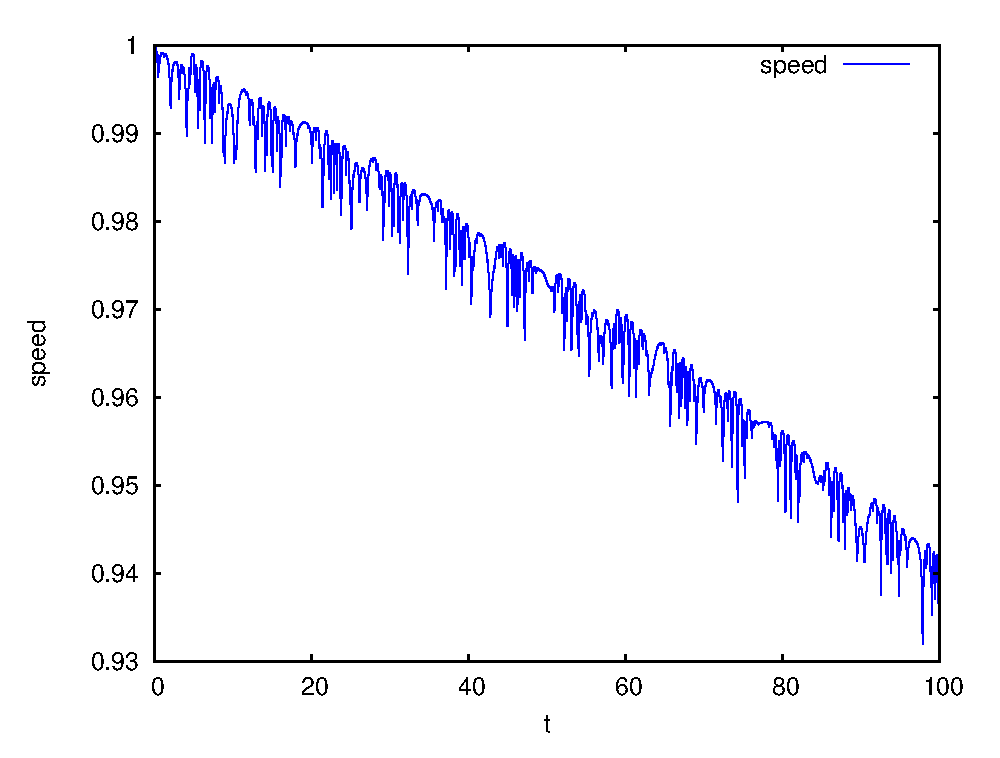
\includegraphics[width=\linewidth]{pic/rol__wrench__speed_of_center_of_mass}\\
            Скорость центра масс
    \end{columns}
    
    \begin{columns}
        \column{0.35\textwidth}
            \centering
            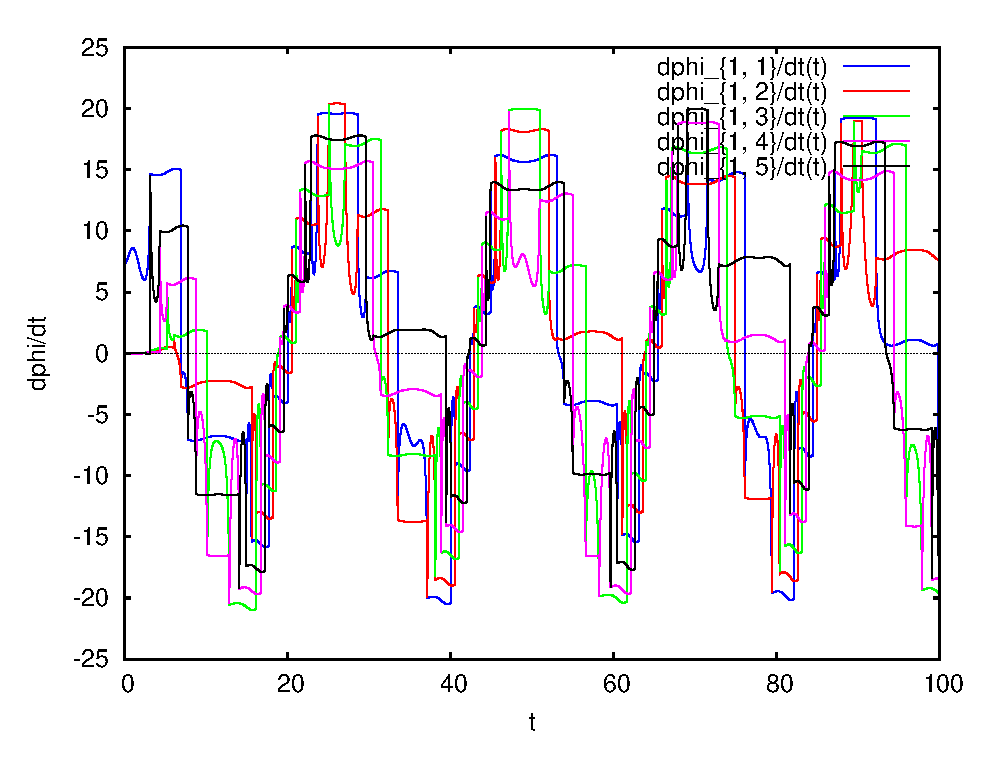
\includegraphics[width=\linewidth]{pic/rol__wrench__velocities_of_rollers_of_wheel_1}\\
            Скорости роликов $\dot{\phi}_{ij}(t)$ на колесе №1
        \column{0.45\textwidth}
            \centering
            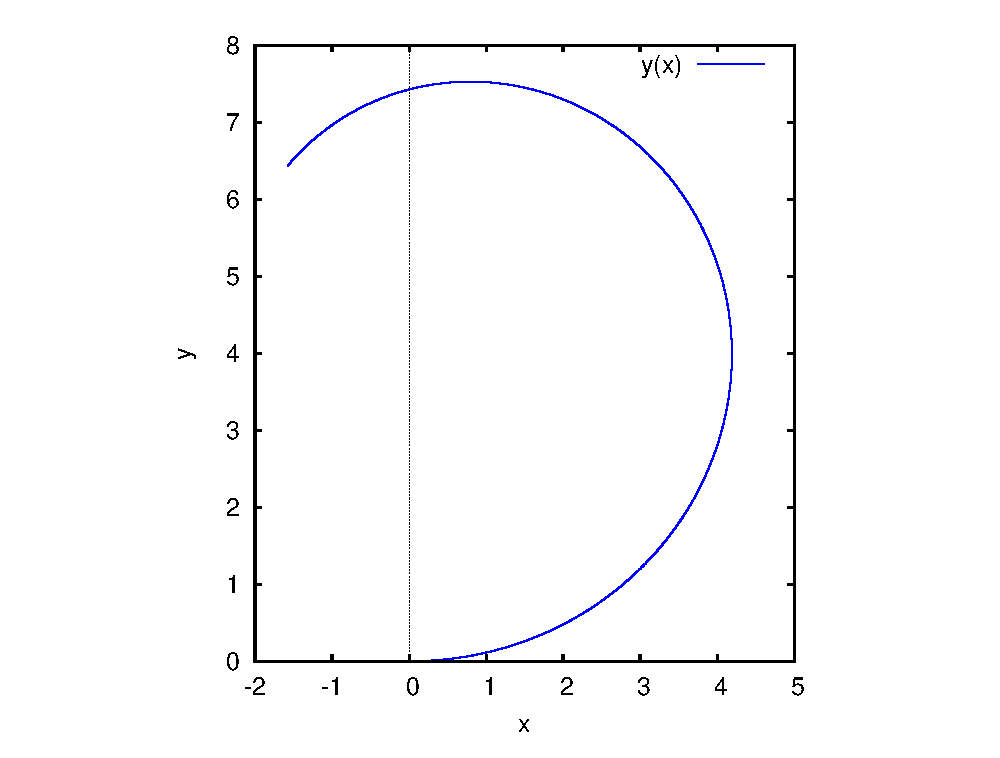
\includegraphics[width=\linewidth]{pic/rol__wrench__trajectory}\\
            Траектория центра масс
    \end{columns}

\end{figure}


{\bf Авторы.}

\begin{itemize}
    \item Герасимов Кирилл Вячеславович (Kirill Gerasimov); 119234, Москва, Ленинские горы, 1Б, 1725; 8 (925) 033-60-79; kiriger@gmail.com;
    \item Зобова Александра Александровна (Aleksandra Zobova); <Ваш домашний почтовый адрес>; 8 (916) 333-19-78; azobova@gmail.com;
\end{itemize}
    
    Кафедра теоретической механики и мехатроники механико-математического факультета МГУ им. М.В. Ломоносова, Москва, Тел.: (495) 939-36-81
    
    On the motion of a symmetrical vehicle with omniwheels with massive rollers
    


\end{document}


